\section{Evaluation experiments and results}
\label{sec:results}

\subsection{Accuracy assessment and bias field correction}
\label{sec:brainweb_evaluation}

\paragraph{Data}
The first experiment demonstrated the accuracy of \gls*{mbis}, and it was conducted
  over the only multivariate dataset included in the \emph{BrainWeb Simulated 
  Brain Database} \citep{cocosco_brainweb:_1997}.
The details of this dataset can found in \autoref{table:data}.
It provides \gls*{t1}, \gls*{t2} and \gls*{pd} realistic
  \gls*{mri}, simulated for only one ``normal'' model presenting a healthy anatomy.
We generated the ground-truth taking the \glspl*{tpm} corresponding to soft tissues
  from the BrainWeb (i.e. \gls*{csf}, \gls*{gm}, glial matter, and \gls*{wm}).
As glial matter and \gls*{gm} are almost indistinguishable (in terms of intensity)
  for the three \gls*{mri} (\gls*{t1}, \gls*{t2} and \gls*{pd}), we merged their
  corresponding \glspl*{tpm} in order to produce a three-class (\gls*{csf}, \gls*{gm},
  and \gls*{wm}) distribution model.
The resulting three \glspl*{tpm} were normalized to sum up to 1.0 at every voxel.
Using the \gls*{map} criterion \eqref{eq:map}, we generated the ground-truth labeling
  (presented in the first row of \autoref{fig:brainweb_hard}).
As it is shown in the same figure, the combination of the three \glspl*{tpm} yields a
  brain mask that was used for brain extraction.

\paragraph{Parameter $\lambda_{\mathcal{N}}$ setting}
We characterized the parameter $\lambda_{\mathcal{N}}$ \eqref{eq:hmrf_energy},
  to set an appropriate default value.
We used the BrainWeb dataset with a noise factor of 5\% and the three available
  inhomogeneity fields (called 0\%, 20\% and 40\% with increasing 
  strength of intensity non-uniformity field).
\begin{figure*}
	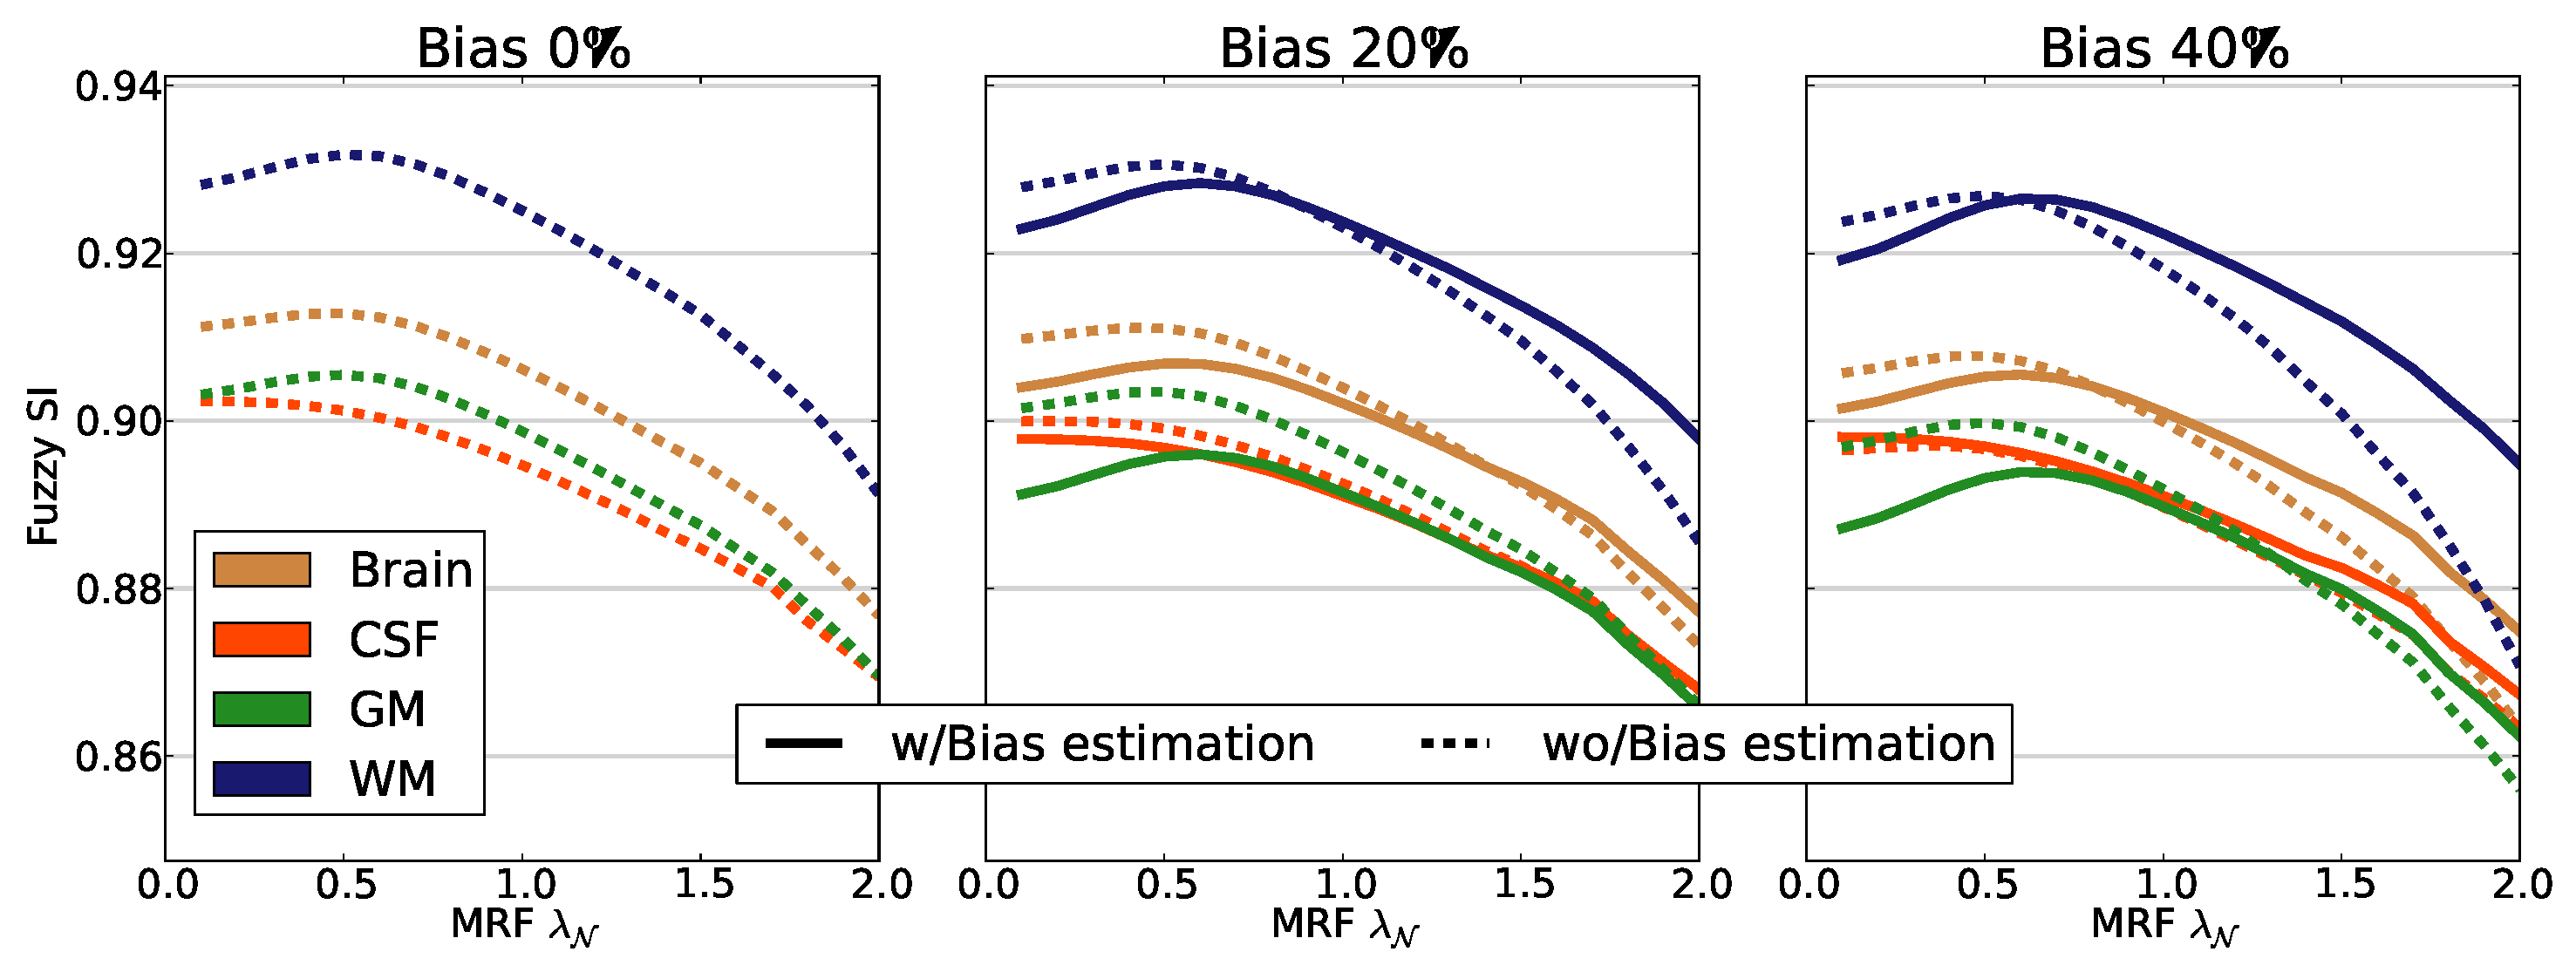
\includegraphics[width=1.0\textwidth]{fig02_mrf_lambda}
	\caption{\textbf{Parameter calibration.} Fine tuning of the parameter $\lambda_{\mathcal{N}}$ 
	\eqref{eq:hmrf_energy}. Dashed lines represent the evaluation without bias estimation and 
	filled lines correspond to the evaluation with bias estimation. The figure shows that the
	optimum value for $\lambda_{\mathcal{N}}$ ranges [$0.55-0.65$].
	}
	\label{fig:mrf_lambda}
\end{figure*}  
From the results shown in \autoref{fig:mrf_lambda}, two conclusions
  can be drawn.
First, $\lambda_\mathcal{N}=[0.55-0.65]$ is consistently the optimum value;
  and second, the bias estimation does not effectively improve the segmentation
  results.
As the channels have independent inhomogeneity patterns, the model is less
  prone to this confounding effect, allowing more flexible \gls*{multivariate_gaussian}
  models without losing sensitivity.
This conclusion is confirmed later, on the visual assessment of the
  estimated bias field maps.
Once $\lambda_\mathcal{N}$ was set, we explored different \gls*{pv} models
  to segment the dataset.

\paragraph{Results}%
The performance test on the synthetic ground-truth was carried out on
  the three available relaxation-time-weighted sequences
  (\gls*{t1}, \gls*{t2}, and \gls*{pd}), with 5\% noise
  and 20\% bias field.
We configured \gls*{mbis} for fully automatic initialization (k-means)
  and $\lambda_\mathcal{N}=0.6$.
Additionally, \gls*{fast} was also used to perform the segmentation using
  its multichannel mode and default settings.
After evaluating numerous configurations, we achieved acceptable results 
  from \gls*{fast} with a four-class model as suggested elsewhere
  \citep{he_generalized_2008}.
We merged the \gls*{tpm} of the fourth class into the one corresponding to \gls*{csf}.
This ad hoc decision was taken after ensuring that the accuracy figures were the
  best we could reach using \gls*{fast}.
The quantitative results shown in \autoref{table:brainweb} indicate a better overall
  performance (row labeled as ``Brain'') of \gls*{mbis} for all the evaluated indices.
\begin{table}[!htbp]
\caption[Quantitative results of the accuracy assessment]{Overlap measured using
  the different indices proposed in \autoref{sec:evaluation_indices}. Boldface font
  highlights the best score for both tools at each overlap index.
  Row labeled as ``Brain'' represents the volume-corrected average of 
  the three detected clusters (\gls*{csf}, \gls*{gm}, \gls*{wm}). Columns contain
  the different indices evaluated (see \autoref{sec:evaluation_indices}):
  \acrfull*{ev_fsi}, \acrfull*{ev_si}, \acrfull*{ev_tpf}, \acrfull*{ev_ef}, and \acrfull*{ev_oc}.
  \label{table:brainweb}}
  \rowcolors{2}{white}{lightgray}
  \begin{tabularx}{1.0\linewidth}{Z|Z|Z|ZZZZ}
\hline
                          &             &  \gls*{ev_fsi}       &   \gls*{ev_si} &  \gls*{ev_tpf} &   \gls*{ev_ef}  &    \gls*{ev_oc} \\ 
\hline  
{\cellcolor{white}}       & \gls*{fast}   &  0.846          &  0.874          &           0.907 &            0.163 &            0.710 \\
\multirow{-2}{*}{Brain}   & \gls*{mbis}   &  \textbf{0.912} &  \textbf{0.940} &  \textbf{0.955} &   \textbf{0.079} &   \textbf{0.871} \\
\hline
{\cellcolor{white}}       & \gls*{fast}   &  0.863          &  0.889          &           0.993 &            0.241 &            0.750 \\
\multirow{-2}{*}{\gls*{csf}}& \gls*{mbis}  &  \textbf{0.900} &  \textbf{0.923} &  \textbf{0.997} &   \textbf{0.163} &   \textbf{0.834} \\
\hline
{\cellcolor{white}}       & \gls*{fast}   &  0.807          &  0.845          &           0.741 &   \textbf{0.014} &            0.632 \\
\multirow{-2}{*}{\gls*{gm}} & \gls*{mbis}  &  \textbf{0.904} &  \textbf{0.939} &  \textbf{0.923} &            0.043 &   \textbf{0.871} \\
\hline
{\cellcolor{white}}       & \gls*{fast}   &  0.868          &  0.888          &  \textbf{0.987} &            0.236 &            0.749 \\
\multirow{-2}{*}{\gls*{wm}} & \gls*{mbis}  &  \textbf{0.931} &  \textbf{0.956} &           0.945 &   \textbf{0.032} &   \textbf{0.908} \\
\hline
\end{tabularx}
\end{table}

Qualitative evaluation using visual assessment and error maps is also reported.
\autoref{fig:brainweb_hard} presents representative views of the error maps
  obtained with the tools under comparison, highlighting regions with remarkable
  differences.
  
\begin{figure}
	\centering
	\includegraphics[width=1.0\linewidth]{fig03-hard_segmentation}
	\caption[Visual assessment of the hard-segmentation results]{The ground-truth is presented on the left column.
	Error maps are presented for \gls*{mbis} and \gls*{fast} (red color represents misclassified pixels).
	Rather than the obvious differences, we highlighted some more subtle examples.
    \label{fig:brainweb_hard}}
\end{figure}
Regarding the \emph{fuzzy} outcome, \autoref{fig:brainweb_fuzzy} presents
  the \glspl*{tpm} obtained with \gls*{mbis} and \gls*{fast}, compared with
  the original ones.
An error map for each tool under testing is also presented, computed as the
  voxel-wise mean squared difference between the three original maps and
  the three maps obtained after segmentation.
\begin{figure*}[!htbp]
	\centering
	\includegraphics[width=1.0\textwidth]{fig04-fuzzy_segmentation}
	\caption[Visual assessment of the fuzzy-segmentation results]
	{First row shows the \glspl*{tpm} of the ground-truth (from left to right:
	\gls*{csf}, \gls*{gm}, \gls*{wm}). Second and third rows present the corresponding
	\glspl*{tpm} obtained with \gls*{mbis} and \gls*{fast}, respectively.
	The extra column represents the mean squared error of the \glspl*{tpm}, 
	normalized by the maximum squared error of both maps.}
	\label{fig:brainweb_fuzzy}
\end{figure*}
 

\paragraph{Bias field estimation}
We conclude the accuracy assessment by studying the performance on estimating
  the bias field.
\autoref{fig:brainweb_results_bias} presents a comparison of the results.
The first row shows the bias field contained by the simulated data from BrainWeb,
  for the \gls*{t1} \gls*{mri}.
The corresponding realizations of bias field for the \gls*{t2} and \gls*{pd}
  images are also available.
The second and third rows present the corresponding estimations obtained with 
  \gls*{mbis} and \gls*{fast}.
Visual assessment is straightforward, as \gls*{fast} did not perform a valid
  estimation of the bias field.
Similar results were obtained for the bias field that affected the \gls*{t2} 
  and \gls*{pd} images.
Even though \gls*{fast} obtained inadequate estimations, segmentation did not
  lose sensitivity dramatically (see \autoref{table:brainweb}), confirming
  that multivariate data are very robust against the different realizations of
  bias field on each channel, as they are independent.

\begin{figure}
	\centering
	\includegraphics[width=1.0\linewidth]{fig05-bias}
	\caption[Comparison of bias estimation]
	{Normalized magnitudes of the reference (first row) and estimated field maps
	are presented (second row is \gls*{mbis}, third is \gls*{fast}),
	for the \gls*{t1} channel.}
	\label{fig:brainweb_results_bias}
\end{figure}

\paragraph{Intra-scan registration} %
The misregistration between the different contrasts stacked as a multivariate image
  is a prominent drawback that hinders multivariate segmentation.
We present in \autoref{fig:segmentation_pitfalls} the characterization of
  the impact of small misalignments between image channels.
More precisely, we translated \gls*{t2} and \gls*{pd} images from their 
  ground-truth location and conducted multivariate segmentation with \gls*{mbis}.
Segmentation results were assessed using the \gls*{ev_fsi} index, and they were
  proven to be quite sensitive to the registration error introduced artificially.
Given that we restricted the analysis only to 3D translations along the Y-axis, a very
  important impact should be expected from other misalignments (as rotations, linear
  transforms of a higher degree, or nonlinear deformations).

\begin{figure}
  	\includegraphics[width=0.95\linewidth]{fig08b_regErr}
    \caption[Intra-subject registration error]{
    	Influence of different combinations of translations
    	between the channels. The figure represents the \acrfull*{ev_fsi}
    	(defined in \autoref{sec:experimental_framework}) versus the absolute
    	displacement.
    	}
    \label{fig:segmentation_pitfalls}
\end{figure}

\subsection{Reproducibility evaluation}
\label{sec:kirby21}
%
\paragraph{Data}
The \emph{Multi-modal \gls*{mri} Reproducibility Resource}
  (also called the \emph{Kirby21 database}) \cite{landman_multi-parametric_2011}
  consists of scan-rescan imaging sessions on 21 healthy volunteers with no history
  of neurological disease.
The database includes a wide range of \gls*{mri} sequences, from which we selected
  \gls*{t1}, \gls*{t2} and \gls*{mt} for segmentation.
The complete database is publicly available online, and details of the \gls*{mri}
  sequences and other information can be found in \autoref{table:data}.

\paragraph{Image preprocessing}
First, all datasets were corrected for inhomogeneity artifacts using \gls*{n4itk} as
  it was necessary to obtain acceptable brain extraction using \gls*{bet}.
Moreover, the use of corrected images as input enabled testing the fully automated
  initialization included in \gls*{mbis}, avoiding the use of atlas information.
\Gls*{t1} images were then enhanced, replacing intensity values
  above the 85$^{th}$ percentile with the local median value.
This filtering removed the typical tail present in the intensity distribution of
  brain-extracted \gls*{t1} images, corresponding to spurious regions remaining
  after skull-stripping.
The second step, after this initial preparation, consisted of correctly aligning
  the different modalities with respect to the reference \gls*{t1} image.
We used \gls*{ants} to register rigidly the \gls*{t2} and \gls*{mt} images to the
  space of the \gls*{t1}.
We visually validated the intra-scan registration of each dataset, as it was
   proven to be an important source of error hindering repeatability in a previous
   experiment (\autoref{sec:brainweb_evaluation}).
   
\paragraph{Segmentation}%
We then used \gls*{mbis} and \gls*{fast} to segment the available datasets
  (a total of 42 datasets from 21 subjects scanned twice), using as input several
  variations of the three available \gls*{mri} sequences (i.e. \gls*{t1}, \gls*{t2},
  and \gls*{mt}).
We do not present a comparison of the repeatability with \gls*{fast} as most of the 
  resulting segmentations from it were not visually acceptable.
Even when the results were visually acceptable, they were not repeatable
  because of the well-known \emph{identifiability} problem \citep{bishop_pattern_2009}.
This problem occurs when a class is correctly detected, but assigned to a different 
  class-identifier, which makes the automatic computation of the evaluation indices
  impossible.
We performed segmentation using \gls*{mbis} with four different combinations of 
  sequences: \gls*{t1} alone, \gls*{t1}-\gls*{t2}, \gls*{t1}-\gls*{mt}, and 
  \gls*{t1}-\gls*{t2}-\gls*{mt}.
The first evaluation considering only the \gls*{t1} channel is the standard
  methodology and reference.
All segmentation trials used a five-class model, where four represented pure 
  tissues (two for \gls*{csf} and one each for \gls*{gm} and \gls*{wm}).
The remaining class fitted the partial volume existing between \gls*{csf} and \gls*{gm}.
We post-processed the \gls*{mbis} results to obtain the probability maps corresponding
  to three-class clustering, as described in \autoref{sec:implementation_details}.

\begin{figure*}[!htbp]
  \centering
  \subfigure[Volume agreement.]{%
  \label{fig:rep_volume}%
  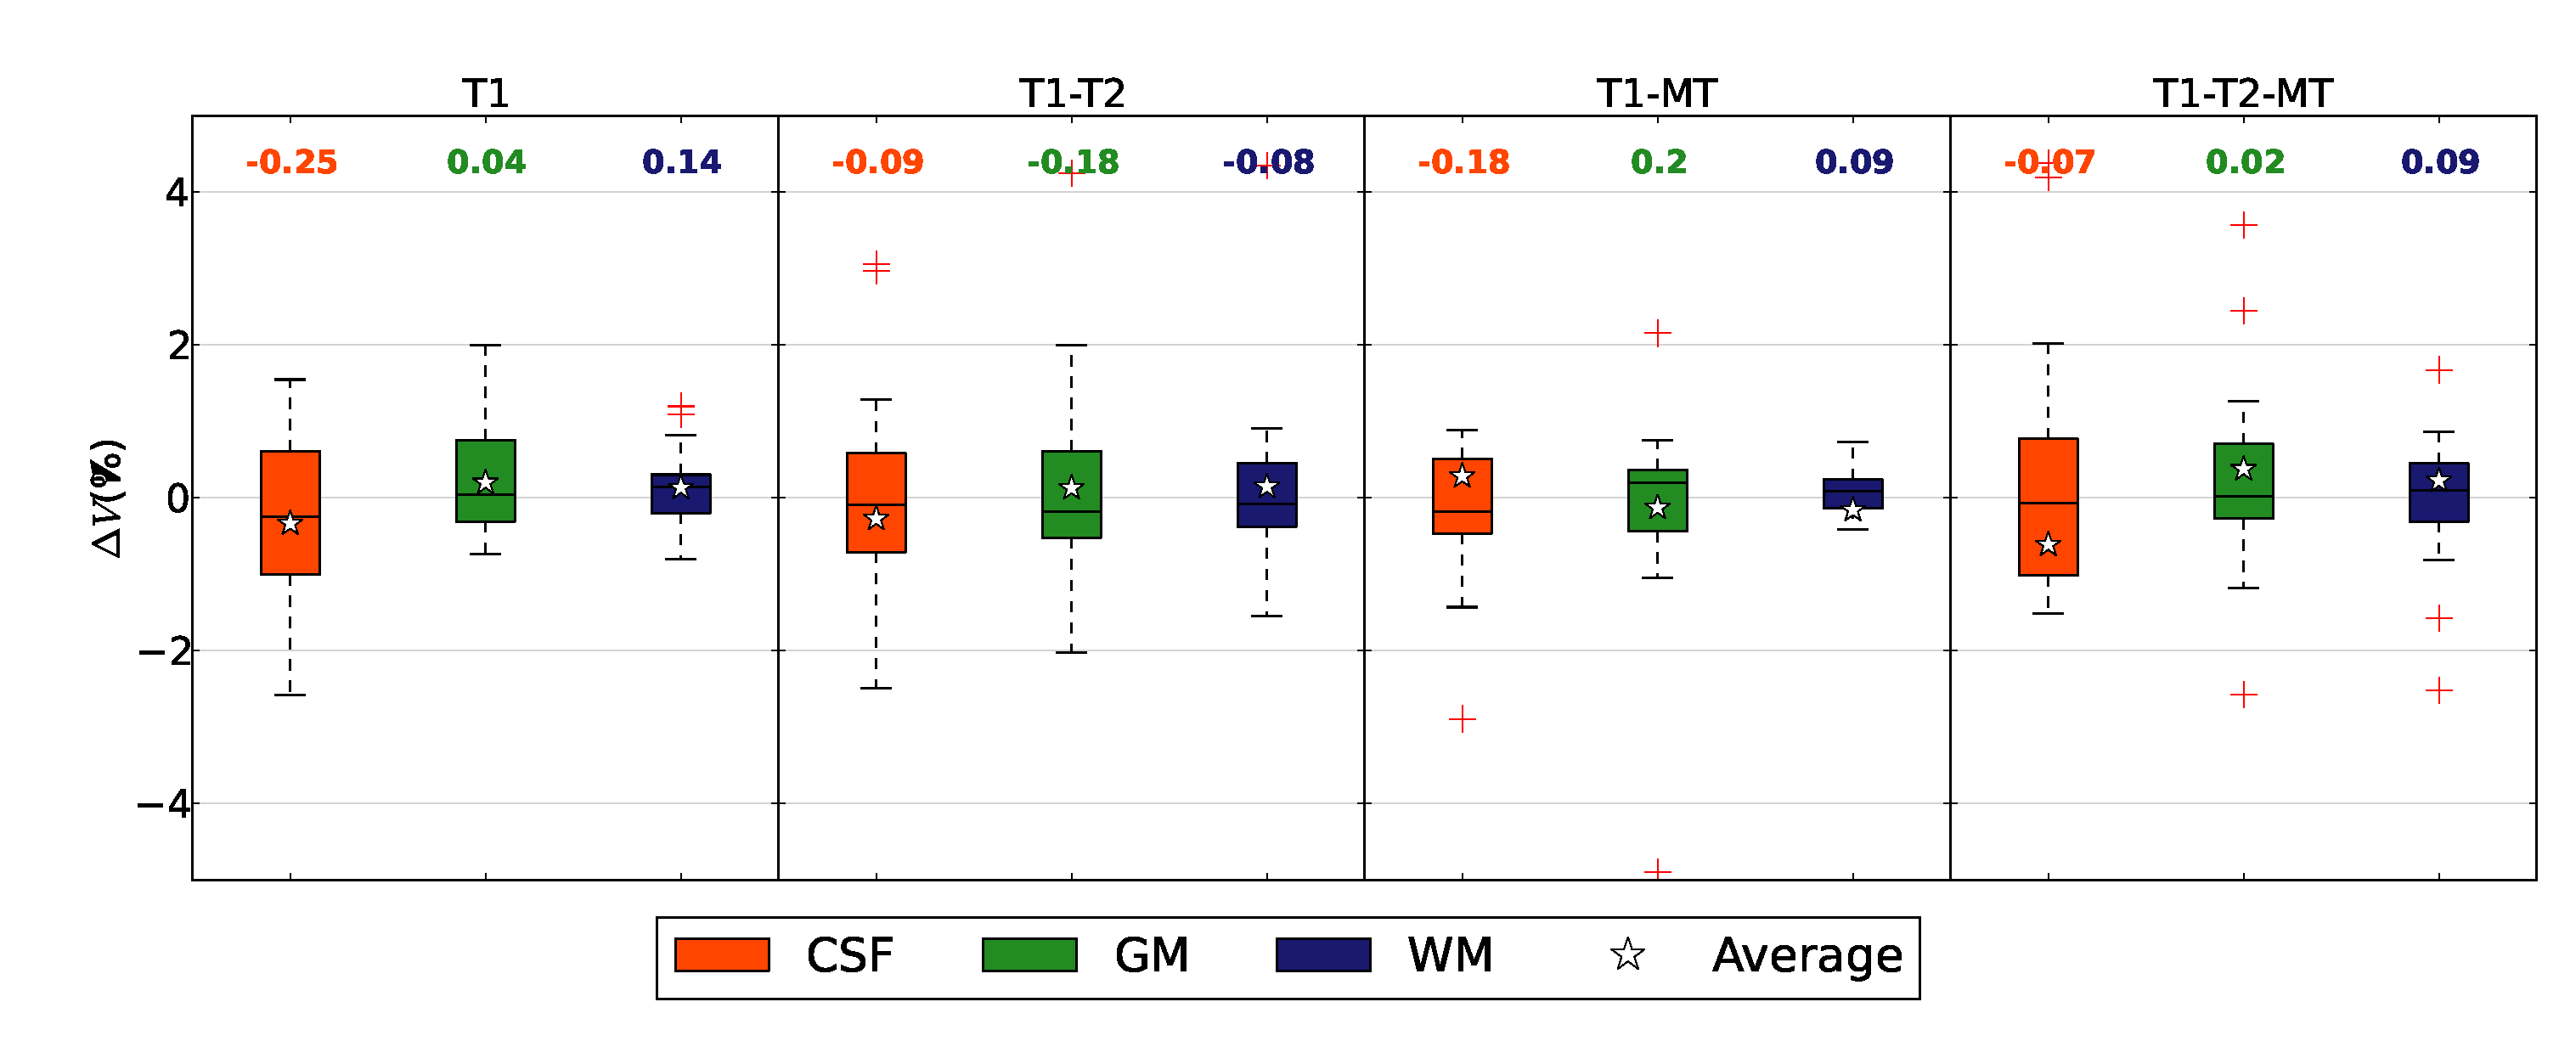
\includegraphics[width=1.0\linewidth]{fig09_k21_vol}
  }\\
  \subfigure[Fuzzy Similarity Index.]{%
  \label{fig:rep_overlap}%
  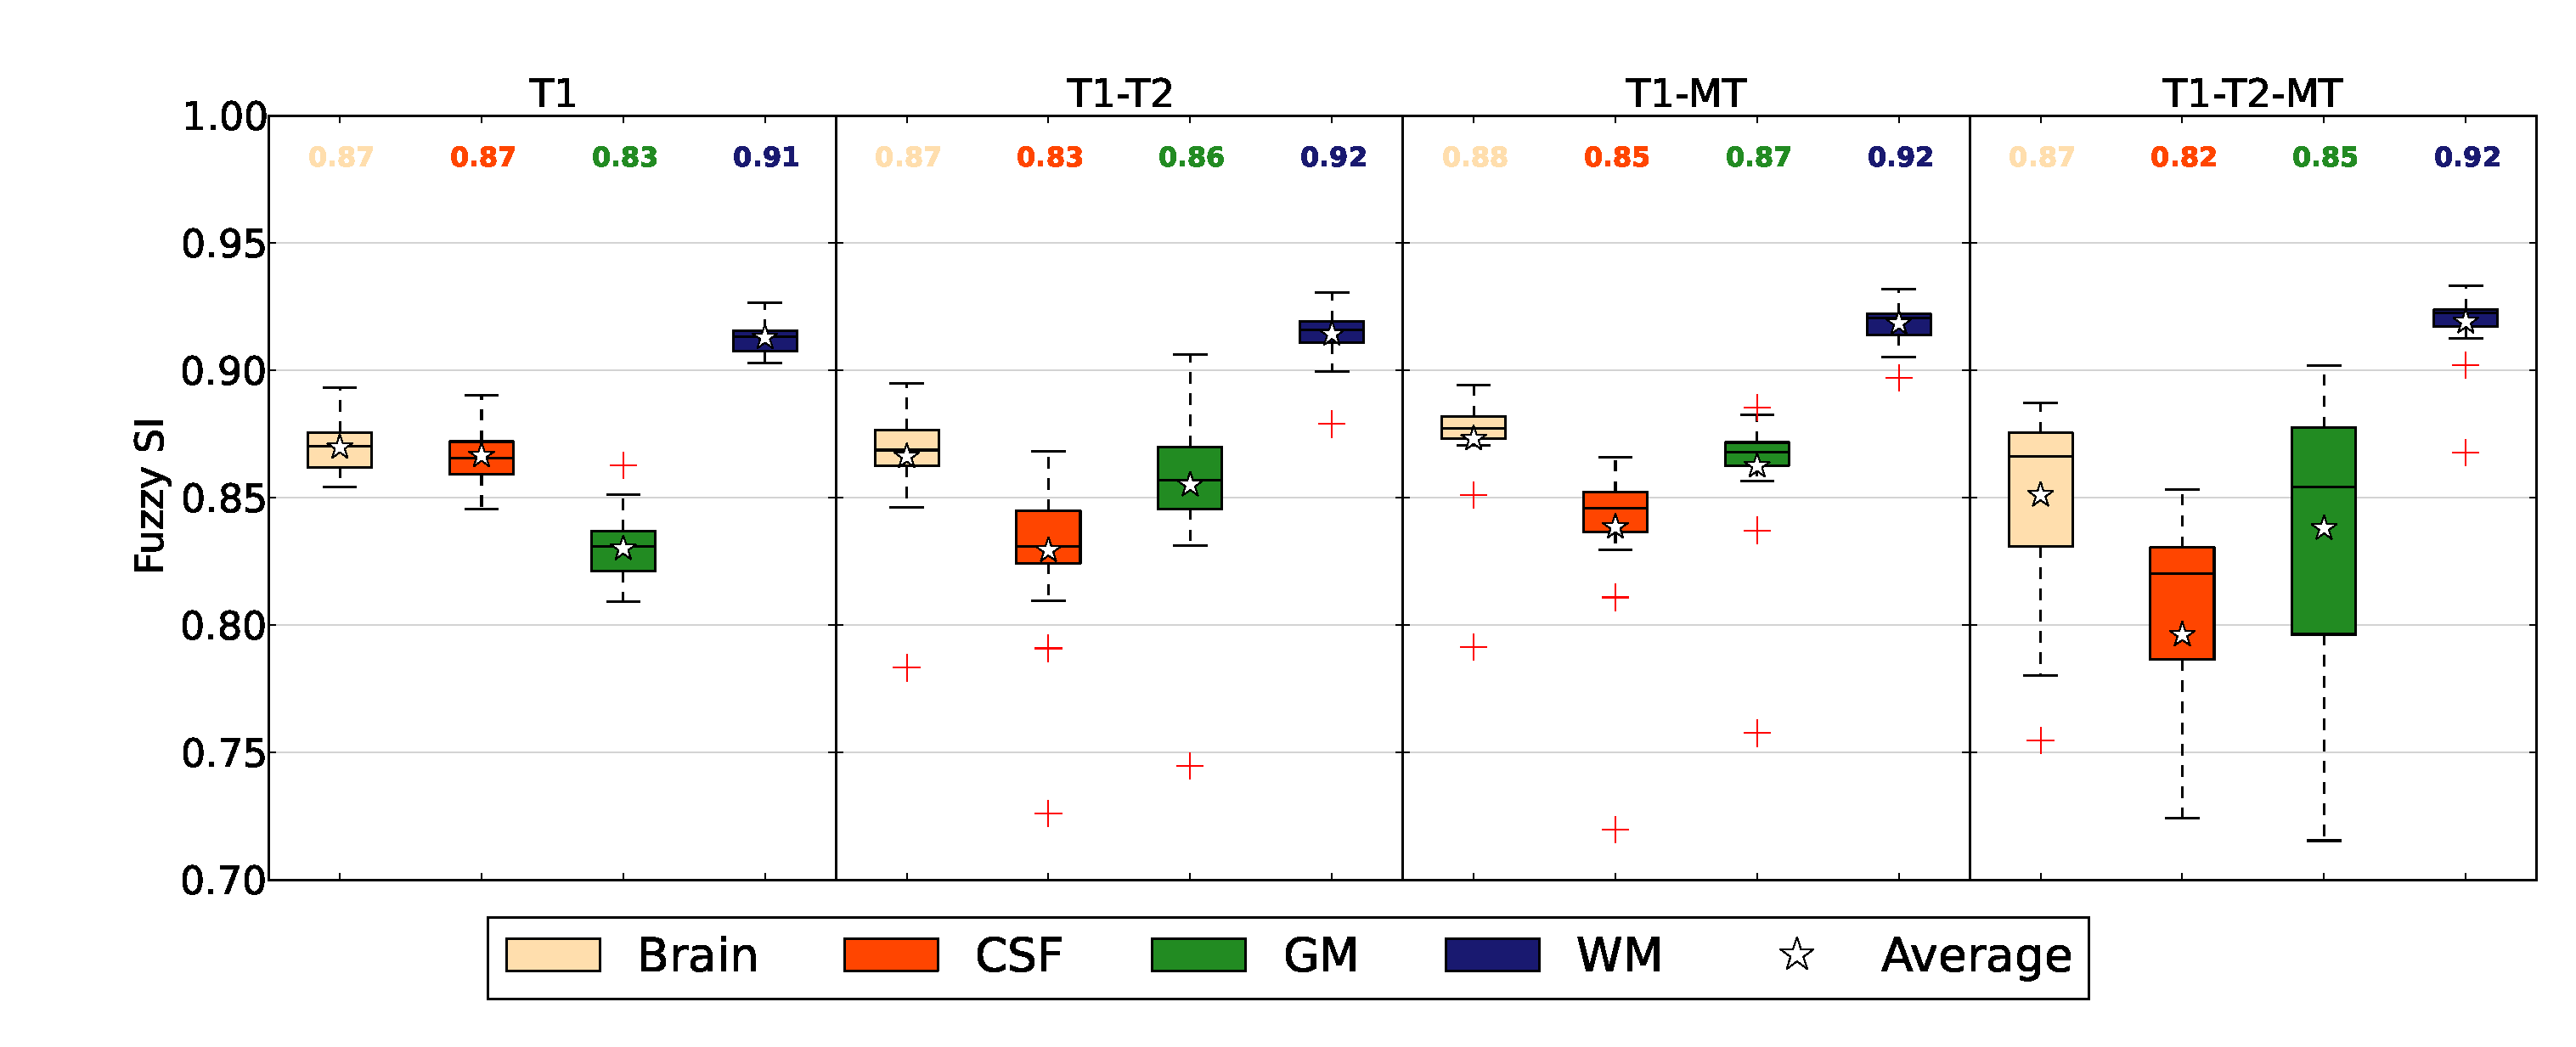
\includegraphics[width=1.0\linewidth]{fig10_k21_ove}
  }
  \caption[Repeatability experiment]{Above each subplot, the \gls*{mri} sequences that
  were stacked to conduct each segmentation are indicated in the title.
  For instance, ``T1'' stands for \gls*{t1} alone, ``T1-T2'' stands for 
  \gls*{t1} and \gls*{t2}, and so forth.
  Inside the plots, the median value of each box is on top in the color of the corresponding tissue.
  \label{fig:repeatability}}
\end{figure*}

\paragraph{Results}
The first experiment consisted of measuring the volume change of each tissue 
 ($\Delta V_{\gls*{csf}}$,$\Delta V_{\gls*{gm}}$,$\Delta V_{\gls*{wm}}$) between the 
 two time points available for each subject (\autoref{fig:rep_volume}).
Bivariate approaches (\gls*{t1}-\gls*{t2} and \gls*{t1}-\gls*{mt}) decreased the volume
  agreement variance, thus providing a more robust outcome than using \gls*{t1} alone.
For the segmentation with three \gls*{mri} components, results were in the same range
  as for \gls*{t1} alone, but presented greater variance.
However, median tissue increments were closer to zero than the 
  monospectral segmentation medians.
The increased variance of results and the appearance of some additional
  outliers when segmenting in multichannel mode may be explained by two
  factors: a) the low quality of some datasets, where motion and gradient
  amplifier failure artifacts were present, and b) the misregistration of data
  between channels.
On one hand, some datasets on the \emph{Kirby21} database presented rather low quality,
  especially some of the \gls*{t2} images.
On the other hand, even though we visually validated intra-scan registration performance,
  some datasets were imperfectly aligned.

The second evaluation consisted of estimating the indices described
  in \autoref{sec:evaluation_indices}, after performing the segmentation
  independently over all of the two scan sessions and the four variations of
  multivariate inputs.
In order to measure the overlap between segmentations of the two scan sessions,
  an ``inter-scan'' alignment was performed by registering the \gls*{t1} image
  of the second scan to the first one with \gls*{flirt}.
The transform was used to resample the segmentation of the second scan input set
  in the space of the corresponding first scan.
\begin{table*}[!htbp]
   \caption[Quantitative results for overlap repeatability experiment]{All these measurements 
   are complementary to the results presented in \autoref{fig:rep_overlap}, and they are 
   computed with the hard segmentation results.
   First column indicates the tissue evaluated, labeling as ``Brain'' the weighted average
   of the other three.
   Second column specifies the \gls*{mri} sequences that were stacked as multivariate input
   (e.g. ``\gls*{t1}-\gls*{mt}'' means that the input feature vector contains samples drawn
   from the \gls*{t1} image as first component and from the \gls*{mt} image for the second).
   Remaining columns contain the different indices evaluated (see \autoref{sec:evaluation_indices}):
   \acrfull*{ev_si}, \acrfull*{ev_tpf}, \acrfull*{ev_ef}, and \acrfull*{ev_oc}.\label{table:rep_overlap}}
   \centering\footnotesize\rowcolors{2}{white}{lightgray}
   \begin{tabularx}{1.0\linewidth}{l|l|ZZZZ}
\hline
 &            &          \gls*{ev_si} &         \gls*{ev_tpf} &           \gls*{ev_ef} &            \gls*{ev_oc} \\
\hline 
{\cellcolor{white}}&\gls*{t1}&0.834$\pm$0.011&0.852$\pm$0.010&\textbf{0.192$\pm$0.016}&0.586$\pm$0.036\\
                    &\gls*{t1}-\gls*{t2}&\textbf{0.851$\pm$0.031}&\textbf{0.883$\pm$0.029}&0.207$\pm$0.051&\textbf{0.624$\pm$0.102}\\
{\cellcolor{white}}&\gls*{t1}-\gls*{mt}&0.840$\pm$0.034&0.873$\pm$0.032&0.221$\pm$0.061&0.590$\pm$0.115\\
\multirow{-4}{*}{Brain}&\gls*{t1}-\gls*{t2}-\gls*{mt}&0.847$\pm$0.036&0.877$\pm$0.037&0.203$\pm$0.044&0.602$\pm$0.134\\
\hline
{\cellcolor{white}}&\gls*{t1}&\textbf{0.800$\pm$0.016}&0.851$\pm$0.016&\textbf{0.277$\pm$0.040}&\textbf{0.499$\pm$0.052}\\
                    &\gls*{t1}-\gls*{t2}&0.754$\pm$0.042&\textbf{0.863$\pm$0.050}&0.434$\pm$0.168&0.339$\pm$0.161\\
{\cellcolor{white}}&\gls*{t1}-\gls*{mt}&0.746$\pm$0.047&0.858$\pm$0.075&0.452$\pm$0.207&0.307$\pm$0.183\\
\multirow{-4}{*}{CSF}&\gls*{t1}-\gls*{t2}-\gls*{mt}&0.739$\pm$0.064&0.814$\pm$0.091&0.388$\pm$0.117&0.269$\pm$0.279\\
\hline
{\cellcolor{white}}&\gls*{t1}&0.771$\pm$0.018&0.773$\pm$0.024&0.233$\pm$0.033&0.404$\pm$0.062\\
                    &\gls*{t1}-\gls*{t2}&\textbf{0.861$\pm$0.051}&0.853$\pm$0.070&\textbf{0.128$\pm$0.064}&\textbf{0.668$\pm$0.150}\\
{\cellcolor{white}}&\gls*{t1}-\gls*{mt}&0.835$\pm$0.057&0.830$\pm$0.080&0.159$\pm$0.105&0.593$\pm$0.168\\
\multirow{-4}{*}{GM}&\gls*{t1}-\gls*{t2}-\gls*{mt}&0.856$\pm$0.055&\textbf{0.867$\pm$0.052}&0.161$\pm$0.087&0.652$\pm$0.159\\
\hline
{\cellcolor{white}}&\gls*{t1}&0.932$\pm$0.006&0.931$\pm$0.012&0.066$\pm$0.012&0.854$\pm$0.014\\
                    &\gls*{t1}-\gls*{t2}&0.937$\pm$0.010&0.932$\pm$0.024&0.058$\pm$0.017&0.865$\pm$0.024\\
{\cellcolor{white}}&\gls*{t1}-\gls*{mt}&0.939$\pm$0.011&0.932$\pm$0.030&\textbf{0.053$\pm$0.017}&0.869$\pm$0.025\\
\multirow{-4}{*}{WM}&\gls*{t1}-\gls*{t2}-\gls*{mt}&\textbf{0.946$\pm$0.007}&\textbf{0.952$\pm$0.014}&0.061$\pm$0.025&\textbf{0.885$\pm$0.016}\\
\hline
\end{tabularx}
\end{table*}
A summary of the indices evaluated over the hard segmentations is shown
  in \autoref{table:rep_overlap}.
For the \gls*{ev_fsi} \eqref{eq:si_index} counterpart, visual plots are presented
  in \autoref{fig:rep_overlap}.
The results are consistent with the conclusion drawn from the previous experiment,
  that is, a slight advantage of two-channel segmentation over classical monospectral
  and three-channel segmentations.
Specifically, the combination of  \gls*{t1} with \gls*{mt} showed better results than
  the remaining choices (despite a few outliers).
This conclusion is supported by recent work studying how \gls*{mt} can improve brain tissue
  segmentation with respect to using \gls*{t1} alone \citep{helms_improved_2009}.


\subsection{Suitability for large-scale studies}
\label{sec:ixi}
\paragraph{Data}
The \emph{IXI dataset} \citep{hill_ixi_2006} is a publicly available database
  containing nearly 600 \gls*{mri} scans of healthy subjects.
The acquisition protocol for each subject includes \gls*{t1}, \gls*{t2} and \gls*{pd}
  images and some other modalities, which we did not consider in our current study.
Additional information about this database can be found in \autoref{table:data}.
From this resource, we discarded those subjects for whom information on their age was not
  available in the demographic spreadsheet distributed along with the IXI dataset.
After this reduction, a total cohort of 585 was selected for the experiment,
  which consisted of measurements of tissue volumes for all individuals to
  illustrate volume change with respect to the subjects' age
  (see \autoref{fig:ixi_regression}).
\begin{figure*}
  \includegraphics[width=1.0\linewidth]{fig11_ixi}
  \caption[Volumetry study upon \emph{IXI dataset}]{Results
    for 584 of 585 subjects are presented, along with the correspondent regression lines.
    \Acrfull*{icv} fraction quantifies tissue volume with respect to the whole-brain
    volume, as defined in \autoref{sec:experimental_framework}.}
  \label{fig:ixi_regression}
\end{figure*}

\paragraph{Image preprocessing}
We focused again on providing a standard processing pipeline, reusing part of the
  workflow defined for the previous experiment.
Firstly, we corrected for bias with the same procedure.
We accomplished the skull-stripping task on the \gls*{t1} image combining the results
  obtained with \gls*{bet} and Freesurfer (\texttt{mri\_watershed})
  for better precision.
\Gls*{t1} images were also enhanced as in the previous experiment.
Finally, intra-subject registrations of \gls*{t2} and \gls*{pd} to the reference 
  (\gls*{t1}) were performed using \gls*{flirt}.

\paragraph{Results}
We computed the \gls*{icv} fraction as defined in \autoref{sec:experimental_framework} from
  segmented data and present results in scatter plots with respect to the subjects' age
  corresponding to each dataset (see \autoref{fig:ixi_regression}).
Among the 585 subjects, segmentation failed in one case, and thus it was removed from the
  computation of the linear regression.
Our results were perfectly aligned with those published previously \citep{taki_correlations_2011,
  abe_sex_2010,mortamet_effects_2005,good_voxel-based_2001,ge_age-related_2002}.
In summary, we captured the linear increase of \gls*{csf} volume and the natural loss of \gls*{gm}
  through aging.
In addition, we perceive a more ``quadratic'' behavior of the \gls*{wm} fraction:
  slightly increasing until an age of approximately 45 years and decreasing thereafter.
As we studied relative \gls*{icv} fractions, this late decrease effect on \gls*{wm} does 
  not imply necessarily a reduction of its absolute tissue volume.
In this regard, we recall that the aim of this third study was not to show the proven 
  relationship between tissue volume and subject age.
We instead demonstrated the aptness of exploiting all of the available data with
  the multivariate approach as a useful improvement of the existing methodologies.
Therefore, we propose \gls*{mbis} as an appropriate tool for this kind of study among others.
